% Discussion

\chapter{Discussion}

With All these results the \gls{tune} can be assumed to be visible and it is then possible to assess the feasibility of the tune measurement using \gls{GPU}. There is still some question around hardware update but the work left to be done can be fairly well estimated.

\section{Observation}

During the three \glspl{MD} we acquired around TODO with both beam and both planes. This data was acquired in XML files and stored on the \gls{CERN} infrastructure. XML was chosen as it is easily accessible by both custom and commercial data analysis software.

Matlab was used as the first tool to check the data and try different algorithm but in the end the software was ready fast enough and flexible enough. Matlab ended to be only used for check and test purpose and all the analysis and discussion is based on the result obtain with the data analysis software described in section~\ref{sec:data_analysis_software}.

\subsection{Without damper}

When the \gls{ADT} is off line there is a clear mark on the tune as shown in Figure~\ref{fig:adt_off}. There is still discussion on is it the tune or just a ripple of the tune but as when the tune is moved the mark is also moving it is safe to assume this is really the tune. Some test could still be made, crosschecking with the \gls{BBQ}, changing the tune and looking in real time.

\begin{figure}[H]
\caption{Spectrogram with ADT off on the 16 October 2012 on vertical beam 1 before the ramp, 6 bunches 10 accumulations}
\label{fig:adt_off}
\centering
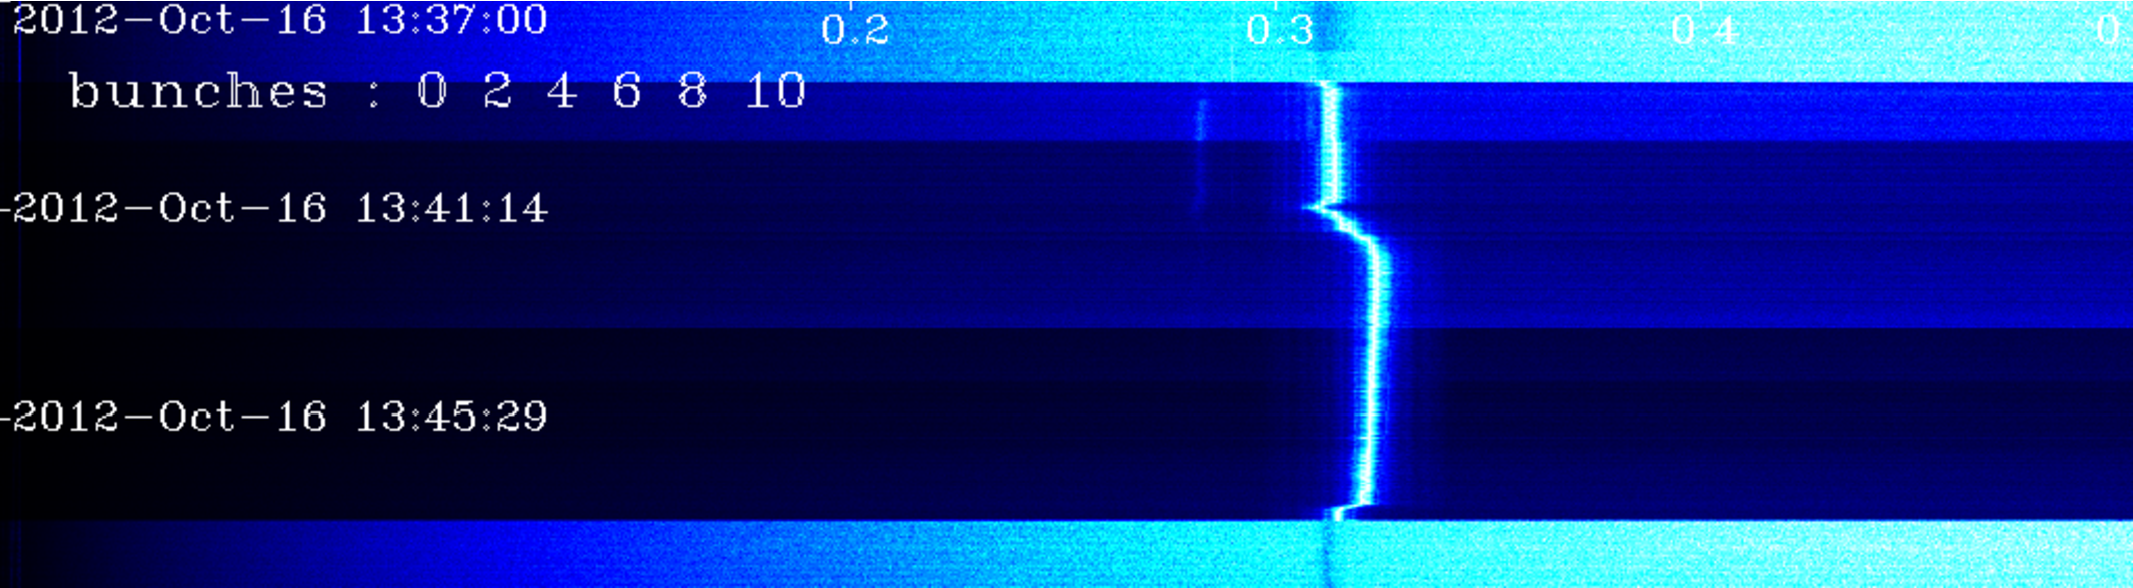
\includegraphics[scale=0.3]{md-121016-vb1-m1-6bunches-10acc-1337-1349-ADT-off.pdf}
\end{figure}

These observations are consistent with the gated-\gls{BBQ} result of 2012 \cite{Valuch12} and show that we can acquire the tune with the \gls{ADT} and get a clear bunch-by-bunch view of the tune even for only one bunch as shown in Figure~\ref{fig:bunch_0_adt_off}.

\begin{figure}[H]
\caption{Spectrogram with ADT off on the 16 October 2012 on horizontal beam 1 before the ramp, 1 bunch (0) 8 accumulations}
\label{fig:bunch_0_adt_off}
\centering
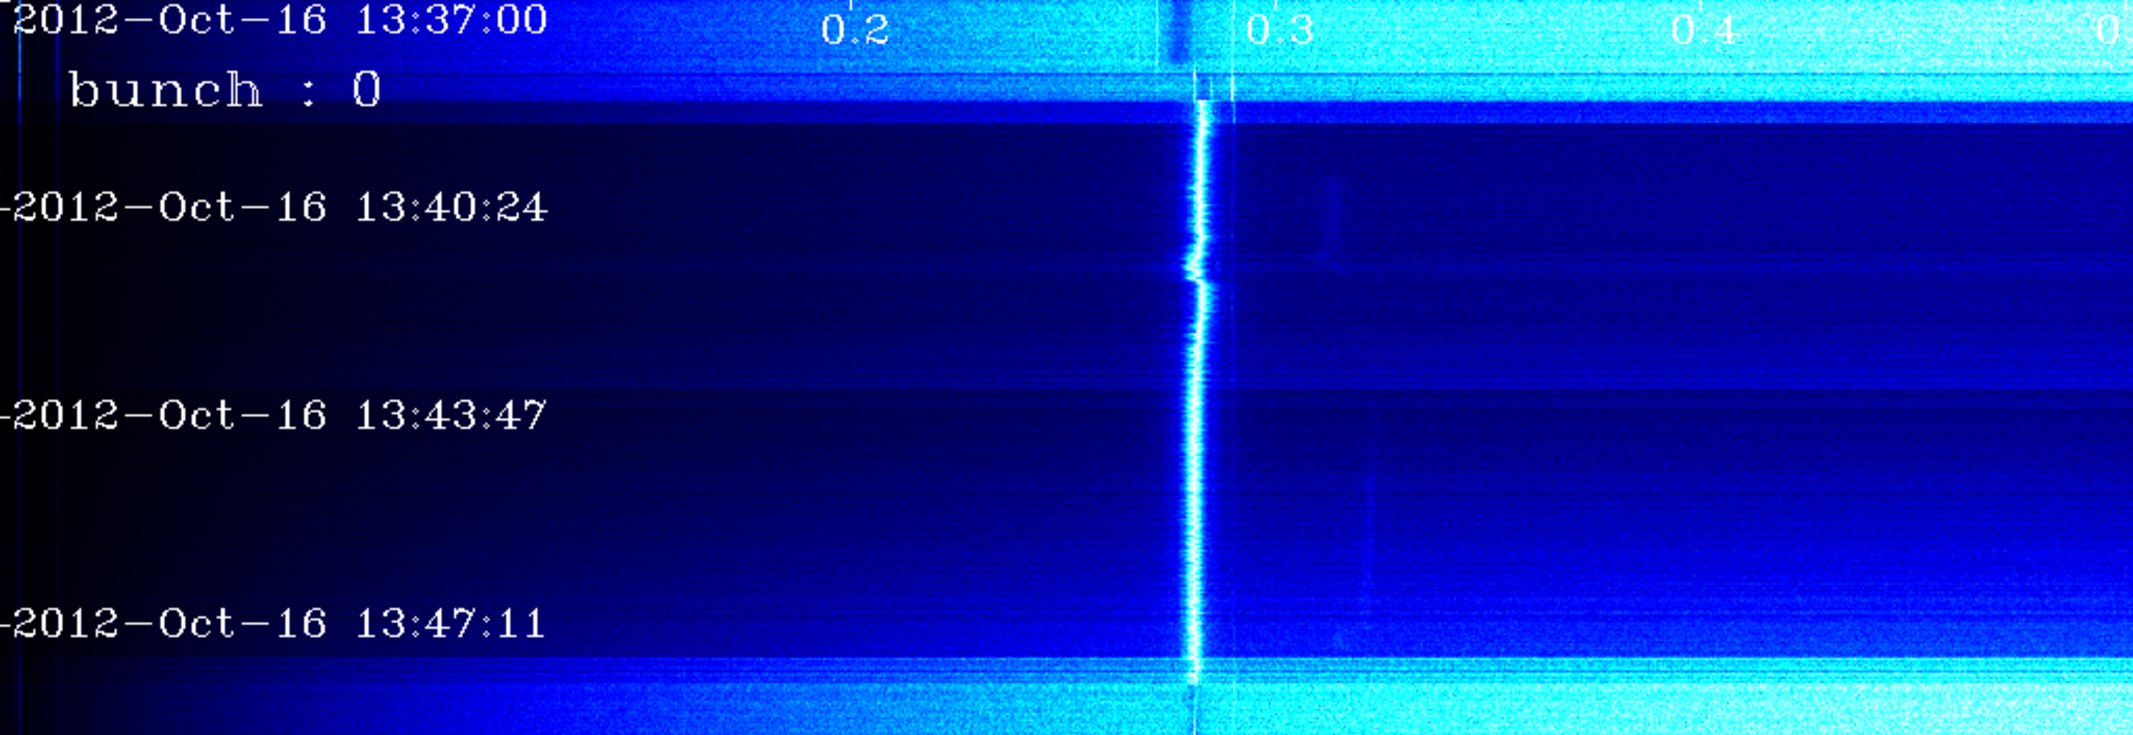
\includegraphics[scale=0.3]{md-121016-hb1-m1-bunch000001-8acc-1337-1349.pdf}
\end{figure}

\subsection{With damper}

When the \gls{ADT} is working the oscillations of the beam are damped by it, as a result the tune is less visible. But we should be able to see the effect of the tune on the damper if the damper is well adjusted to the beam. This mean that we should see a clear gap in the frequency around the tune frequency (or at the frequency the damper is less working, frequency that should correspond to the tune).

This correspond to the spectrogram we see during operation as shown in Figure~\ref{fig:ramp}. We also see in this figure the ramp that lead to collision, before putting the beam in collision we do a squeeze (operation during witch we compress the beam size in the interaction points, where the experiments are). The squeeze is changing the tune and we can see it on the spectrogram around 14h03 on the figure \ref{fig:ramp}.

\begin{figure}[H]
\caption{Spectrogram with damper working on the 16 October 2012 on vertical beam 1 during the ramp, 6 bunches 10 accumulations}
\centering
\label{fig:ramp}
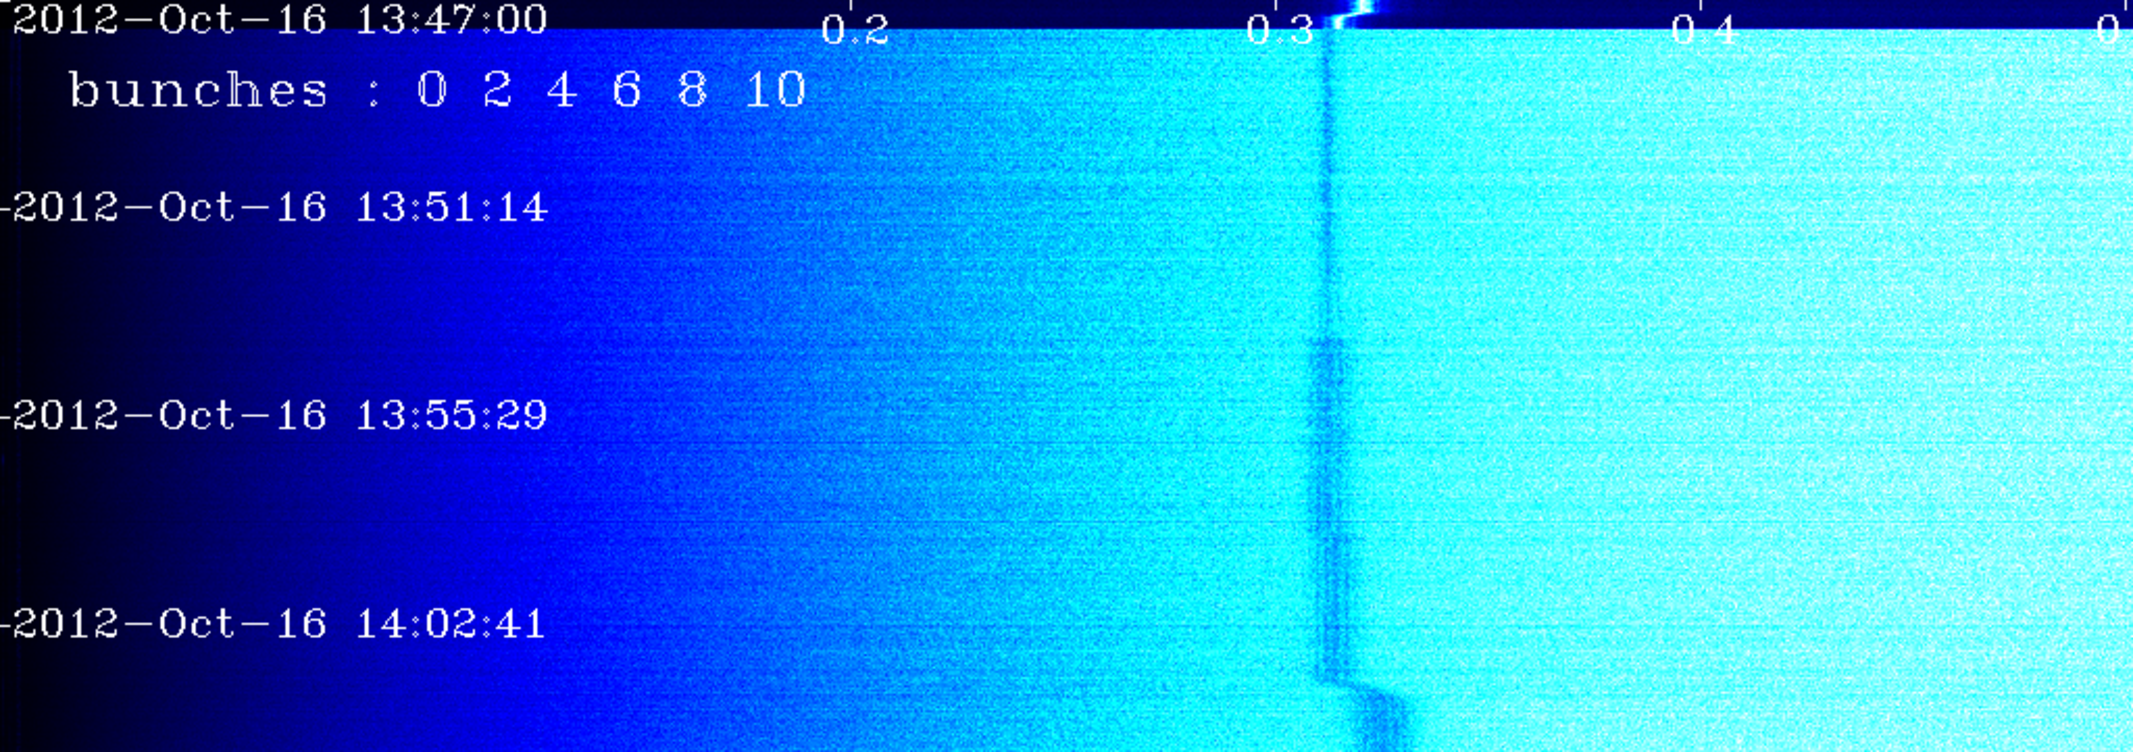
\includegraphics[scale=0.3]{md-121016-vb1-m1-6bunches-10acc-1347-1405-ramp.pdf}
\end{figure}

This could give us a good acquisition of the tune during operation even when \gls{ADT} is on. This acquisition could be made bunch-by-bunch so we could correct position of bunches that are not well on tune. The question that is still up is how much is it sensible to the way the \gls{ADT} is set up. This has still to be tested in the machine by moving the tune while the \gls{ADT} is in operation and see if the acquisitions follows the tune.

\section{Data flow}

As the hardware is not present yet, the time and bandwidth of the whole system has to be estimated to see if it is doable in the constraint we have and that were exposed in the introduction. Estimation of the bandwidth and data flow is shown in Figure~\ref{fig:data_flow}.

\begin{figure}[H]
\caption{Acquisition data flow}
\label{fig:data_flow}
\centering
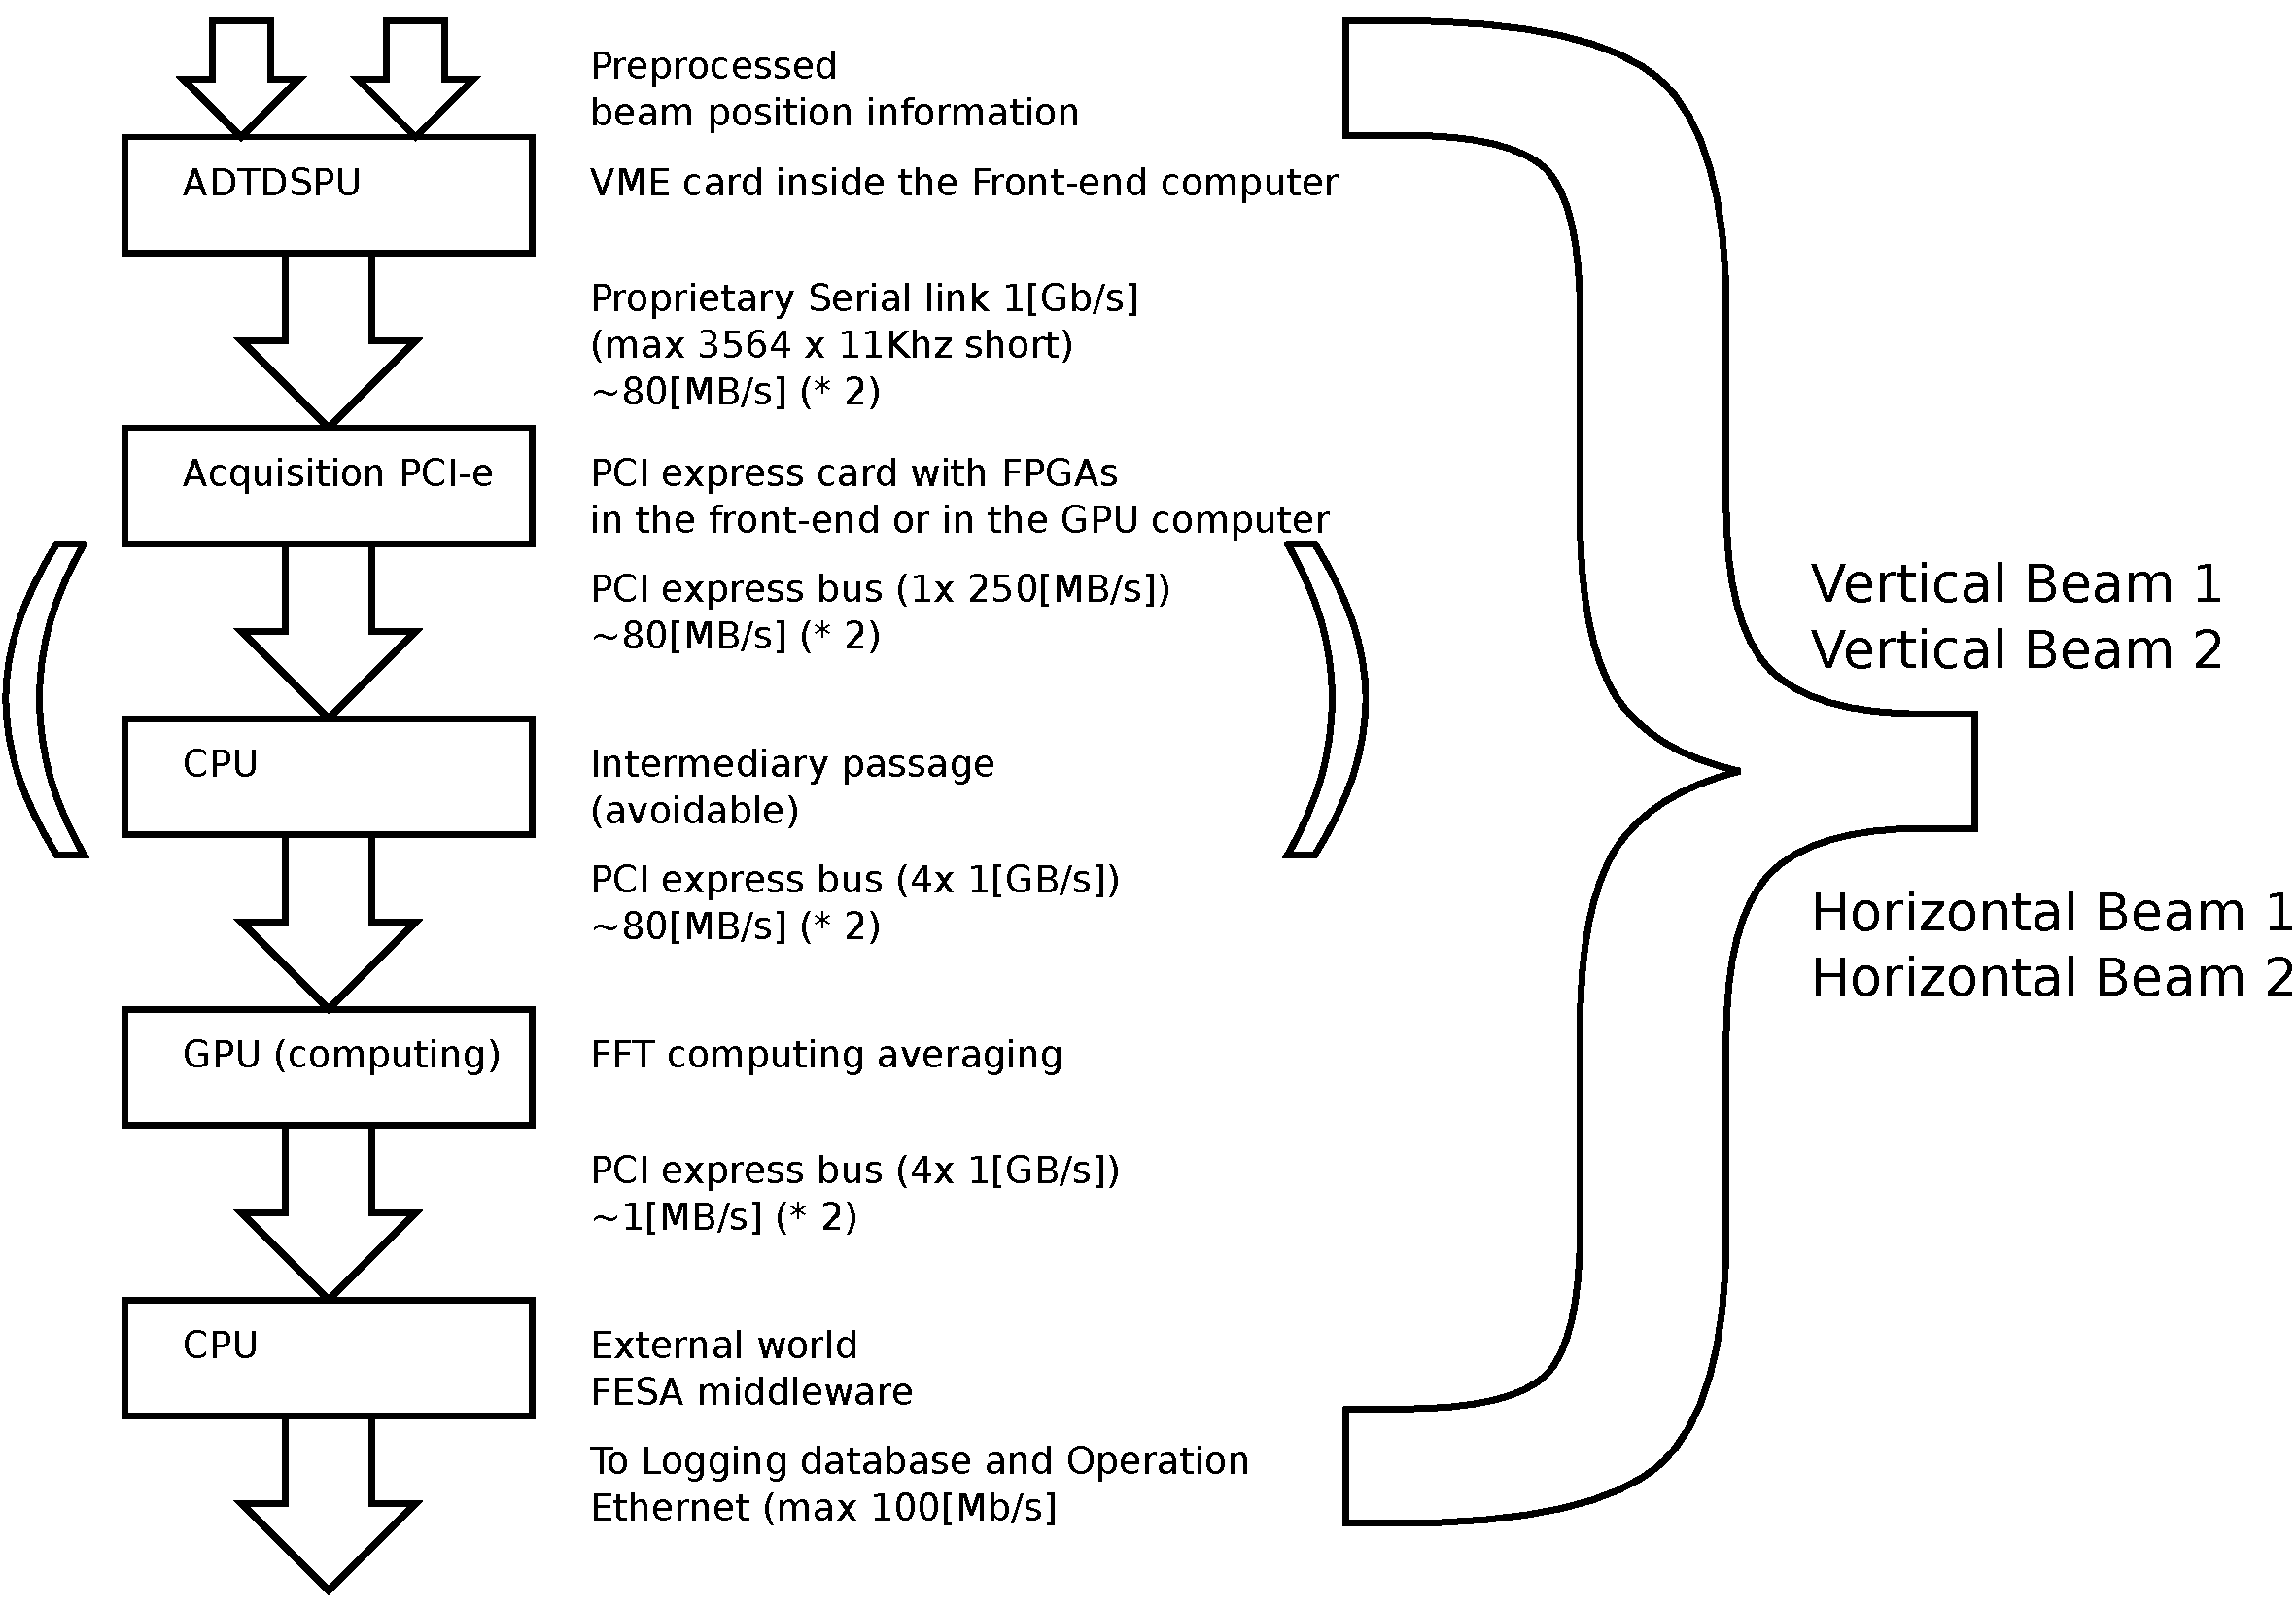
\includegraphics[scale=0.3]{dataflow.pdf}
\end{figure}

The data has to move from the acquisition card to the GPU by a series of steps, first from the card to the PCI crate (the one who contain the actual \glspl{GPU}). The problem being that the acquisition card is a \gls{VME} card and the VME bus is too slow to allow the full data to be streamed to the CPU. This will use the Giga-bit serial link already present on the VME card. A receiver card will then receive the data in the PCI crate and send it either directly to the \gls{GPU} memory or to the \gls{CPU} and then to the \gls{GPU} memory. Then the \gls{GPU} will make the computations necessary for the tune measurement and will copy back to the \gls{CPU} that will use the normal Ethernet connection to stream it back to operation.

\section{Hardware}

The present hardware is not allowing to acquire all the \glspl{bunch} of the machine and is in fact limited by constraints of the \gls{VME}. We have to upgrade various part of the hardware and to add the new computing device in order to be able to make on-line computation of the tune.

\subsection{ADT Acquisition boards}

The ADTDSPU card will be redesigned and remade during the long shutdown 1 (LHC upgrade from beginning of 2013 to 2015). It will be an upgrade of the whole card with tune measurement and other needed features in mind.

\subsection{Serial link interface}

Serial link receiver has to be chosen and put into place in the new computing device to be able to receive the data and pass them to the \gls{GPU}. This card has to be fast enough to get the serial data from the serial link that comes from the ADTDSPU, have a PCI-express interface and \gls{SFP} interface on the front panel. It should also have a fast FPGA to de-serialize the bunch positions and send them to the PCI-express bus. To be able to communicate with the CPU, Linux drivers (with sources) have also to be present.

A market survey revealed that commercial cards can fill up our needs.

\begin{figure}[H]
\caption{Nallatech PCIe-180}
\label{fig:nallatech}
\centering
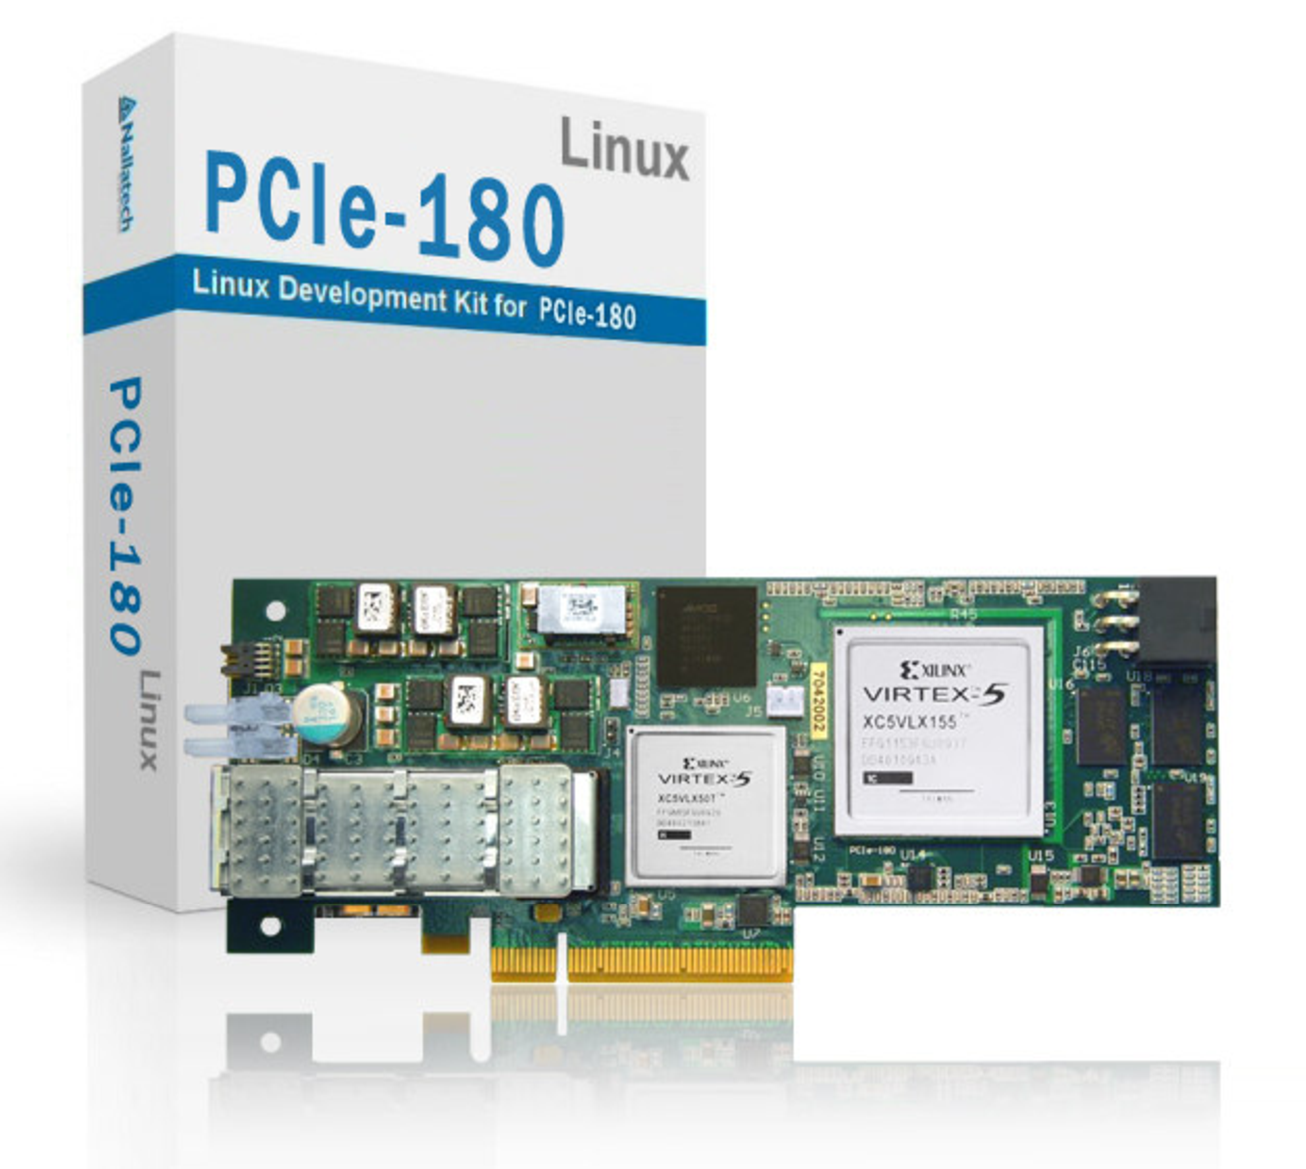
\includegraphics[scale=0.3]{Nallatech_PCIe-180.pdf}
\end{figure}

\gls{CERN} also propose some card that are done by \gls{CO} and can also make a good match.

\begin{figure}[H]
\caption{CERN Simple FMC carrier (SPEC)}
\label{fig:spec}
\centering
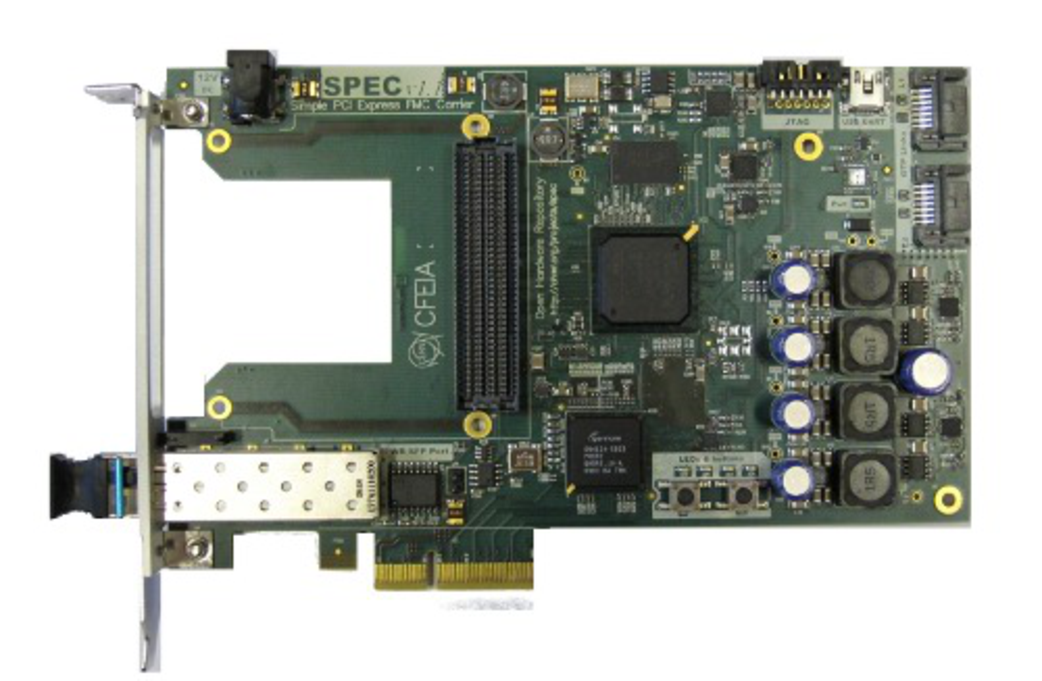
\includegraphics[scale=0.3]{spec_top.pdf}
\end{figure}

Table~\ref{tab:receiver_cards} show the different commercial and CERN solutions.

\begin{table}[H]
\caption{PCIe Giga bit link serial receiver card candidates}
\label{tab:receiver_cards}
\centering
\begin{tabular}{|ll|c|l|c|}
\hline
Name & Manufacturer & SFP & FPGA & Drivers \\
\hline
\hline
SPEC & CERN & 1 & Spartan-6 & yes \\
\hline
Virtex-5 LXT ML555 & Xilinx & 2 & Spartan-5 & no \\
\hline
Xilinx Virtex 6 & Hitech Global & 2 & Spartan-6 & no \\
\hline		
PCIe-287N & Nallatech & 4 & Kintex-7 * 2 & yes \\		
PCIe-180 & Nallatech & 2 & Virtex-5 & yes \\
\hline
\end{tabular}
\end{table}

\subsection{GPUs}

We need a computing device with at least 2 PCIe slots, one for the serial link receiver and one for the \gls{GPU} card. It should be some standardized crate with a powerful \gls{CPU} and possible expansion. Place has to be checked in SR4 to check if there is enough space for full crate or we have to take lighter crates.

\section{Software}

Some software upgrade and redeployment is still necessary before the operational version is fully commissioned.

\subsection{Drivers}

The drivers for the \gls{ADT} acquisition card will need some update, changing the memory map and adjusting the drivers for the control registers. This should be quite straightforward.

A driver for the Serial link receiver card will be needed, either, if we use one that is made inside \gls{CERN} we can have it made by the control group (CO). Or in case we buy an off the shelf solution we will have to make the driver ourself using the driver framework and the tools we have.

\subsection{OpenCL}

The present \gls{OpenCL} code is able to compute the \gls{FFT} but we could try other algorithms in the future including hardware accelerated \gls{SVD}. This would ask some new \gls{OpenCL} development.

\subsection{Front-end}

Developing new software to control the new hardware are needed, the ADTDSPU board is going to be changed and we are going to build a new computing front-end with a custom serial link receiver and a \gls{GPU}. So new drivers and a software to stream data from the receiver card to the \gls{GPU} will be needed.

\section{Intermediate and Final setup}

A normal computer with a decent \gls{CPU} can be estimated to cost around 2'000 SFR and a top \gls{GPU} is around a 1'000 SFR. The reciever card should be in the same value band.

In case we have to move to rackable \gls{CPU} the price can go up to around 10'000 SFR per crate this is still much cheaper than a \gls{VME} crate and custom cards.

\subsection{First prototype}

First prototype will be a normal computer with the receiver card and a \gls{GPU} card. The idea is to test the hardware, and decide on the final setup.

This test will be made on the \gls{ADT} test setup and will be fed from the new version of the \gls{ADTDSPU} card.

\subsection{Final version}

At \gls{LHC} restart four crates will be deployed in SR4 (the ADT Faraday cage). One for each ring and for each plane, the test crate may be moved as well to be used on the test acquisition crate.